\chapter{\IfLanguageName{dutch}{Stand van zaken}{State of the art}}%
\label{ch:stand-van-zaken}

% Tip: Begin elk hoofdstuk met een paragraaf inleiding die beschrijft hoe
% dit hoofdstuk past binnen het geheel van de bachelorproef. Geef in het
% bijzonder aan wat de link is met het vorige en volgende hoofdstuk.

% Pas na deze inleidende paragraaf komt de eerste sectiehoofding.
Om dit onderzoek tot stand te brengen, is er nood aan bepaalde informatie, waaronder over AI-technieken en vermoeidheid zelf. Nadien wordt dit alles verwerkt om het probleem aan te pakken.

\section{Vermoeidheid}
De verkeersveiligheid heeft een grote last van vermoeidheid en slaperigheid. In de literatuur is de definitie van vermoeidheid en slaperigheid anders en bestaat er eigenlijk geen duidelijk onderscheid tussen beide \autocite{RiguelleGoldenbeld}.

Vermoeidheid verwijst naar een weerstand die veroorzaakt wordt door uitputting. Dit heeft het gevolg dat de taken minder efficiënt worden uitgevoerd. Dit kan zowel fysiek (bijvoorbeeld na het sporten of intensief werken) als mentaal zijn (na een veeleisende intellectuele, mentale of psychologische activiteit). Vermoeidheid zorgt er voor dat de taak minder snel wordt afgemaakt of dat de energie zodanig laag ligt dat er aan de volgende taak niet begonnen wordt.

Slaperigheid verwijst naar de moeite om nog wakker te blijven. Het is gekoppeld aan de biologische slaap-waak proces volgens het circadiaan-ritme. Het circadiaan-ritme is een endogene, regelbare schommeling van ongeveer 24 uur (van Latijnse `circa-diem` - ongeveer een dag) van verschillende biologische systemen in het hele lichaam \autocite{Gianni2018}. Slaperigheid heeft dus geen rechtstreeks verband met de uitvoering van een activiteit. Doordat ons menselijk lichaam beschikt over een 'slaapmodus', dit is voornamelijk tussen middernacht en 6 uur, neemt de alertheid bijgevolg af. Dit komt doordat het lichaam, op een cyclus van 24 uur, meer slaap nodig heeft dan op andere momenten.

Hoewel slaperigheid en vermoeidheid logisch niet synchroon verlopen, worden ze vaak gezamenlijk behandeld in de literatuur vanwege hun overeenkomstige gevolgen. Deze twee aparte gevallen kunnen ook tegelijkertijd voorkomen bij iemand. Om het eenvoudig te houden, wordt 'vermoeidheid' waargenomen als slaperigheid.

\section{Oorzaken van vermoeidheid}
Er zijn vijf algemene factoren, namelijk: de tijd besteed aan een taak of werk, slaaptekort, bioritme, monotonie van een taak en individuele kenmerken, die vermoeidheid veroorzaken \autocite{Brown}.
\subsection{De tijd besteed aan een taak of werk}
Eén van de mogelijke oorzaken is de tijd die iemand besteed aan een bepaalde taak of werk. De meeste mensen voelen de eerste symptomen van fysieke vermoeidheid na ongeveer 2 à 3 uren aaneengesloten autorijden \autocite{RiguelleGoldenbeld}.
\subsection{Slaaptekort}
Een slaaptekort kan chronisch of acuut zijn \autocite{VanSchagen2003}. Een chronisch slaaptekort kan veroorzaakt worden door gevolg van te weinig slaap over een lange periode. Men heeft gemiddeld nood aan 8 uur slaap. Echter is het ook van belang dat er goed geslapen wordt. Er kunnen regelmatige verstoringen optreden tijdens het slapen, wat ook leidt tot een chronisch slaaptekort. Een acuut slaaptekort komt ook door het te weinig slapen, maar is minder structureel. Na één slechte of korte nacht, wordt er al gesproken van een partieel acuut slaaptekort. Een volledig acuut slaaptekort komt pas voor indien er in de gehele 24-uursperiode niet geslapen is.
\subsection{Bioritme}
Het bioritme regelt het slaap-waakritme van de mens. Dit is bij iedereen anders. Het hangt dus samen met de dagelijkse slaapcyclus. Dit betekent dat de mens in de ochtend minder behoefte heeft aan slaapt dan op andere tijdstippen. Wanneer de tijd richting middernacht gaat, zal het bioritme meer nood hebben aan slaap. Soms zit er geen consistentie in het bioritme, bijvoorbeeld wanneer iemand nachtdienst heeft.
\subsection{Monotonie van de taak}
Vermoeidheid kan zich ook vormen doordat men een monotone taak uitvoert. Een taak is monotoon wanneer prikkels ontbreken, verandering erg voorspelbaar is of er een hoge maat van herhaling is \autocite{DaCoTA}. Het rijden op een autosnelweg met weinig verkeer en verandering van omgeving kan men zien als een monotone taak. Uit een experimenteel onderzoek is ook gebleken dat de monotonie van een rijtaak na verloop van tijd tot een slechtere rijprestatie leidt.
\subsection{Individuele kenmerken}
Tenslotte hebben individuele kenmerken ook een invloed op de vermoeidheid. Deze factoren, zoals leeftijd, medische conditie, het gebruik van alcohol, geneesmiddelen of drugs, beïnvloeden hoe vatbaar iemand is voor vermoeidheid en hoe goed ze er mee kunnen omgaan \autocite{VanSchagen2003}. Zo zijn oudere mensen, die last hebben van een slechte lichamelijke conditie, vaak sneller vermoeid. In tegenstelling tot tieners, die extra vatbaar zijn voor vermoeidheidseffecten door alcohol, drugs en te weinig slaap.

\section{Verband met verkeersveiligheid}
\subsection{Invloed op het rijgedrag}
Het effect van vermoeidheid op verkeersveiligheid is in verschillende studies onderzocht. Volgens deze studies leidt vermoeidheid achter het stuur tot een aantal negatieve effecten op verkeersgedrag \autocite{RiguelleGoldenbeld}. Deze bestaan uit een tragere reactietijd, verminderende oplettendheid en verwerking van informatie en slechter sturen \autocite{Bartlett,Friswell2008}. 

Volgens onderzoek is de rijprestatie van bestuurders na 17-19 uur slaapdeprivatie slechter dan die van bestuurders met een BAC (bloed-alcohol percentage) van 0.5\%, wat de wettelijke grens is in de meeste Europese landen en Australië \autocite{Williamson2000}. Onderzoek van Dawson \& Reid (1997) geeft aan dat de rijprestatie afneemt na 16 uur slaapdeprivatie en dat 21 uur leidt tot een verminderde rijprestatie die gelijk is aan een BAC van 0.8\%, wat het wettelijk limiet is in Engeland, de Verenigde Staten en Canada \autocite{Dawson1997}.
\subsection{Gevolgen in termen van ongevallen}
De prevalentie van vermoeidheid en de impact dat het heeft op ongevallen, is niet makkelijk te meten \autocite{Diependaele2015}. Dit komt doordat er geen betrouwbaar meetprotocol bestaat. Mensen die in een ongeval terecht komen, geven vaak ook niet toe dat het door de vermoeidheid komt dat het heeft plaatsgevonden. De gegevens uit het "100 Car Naturalistic Driving"-onderzoek tonen aan dat rijden als men moe is, leidt tot een vier keer meer risico op een ongeval \autocite{Klauer2006}.

Wetenschappelijke schattingen, gebaseerd op diepgaande analyses van de verkeersongevallen, geven aan dat 10 tot 15\% van de ongevallen te maken zou hebben met vermoeidheid \autocite{VanSchagen2003}. Een andere schatting zegt dat ongeveer 20 tot 25\% van de ongevallen op Europese wegen te maken heeft met vermoeidheid \autocite{Akerstedt2013}. \textcite{Horne1995} schatten dat vermoeidheid de oorzaak is van 16\% voor de ongevallen op stadswegen en 20\% op autosnelwegen. Een recentere studie van dezelfde auteurs \autocite{Horne1999} bevestigt dat de ongevallen door middel van vermoeidheid vaker gebeuren op autosnelwegen doordat rijden op een autosnelweg gezien wordt als een monotone taak. 
Gebleken uit een analyse van over 600 ongevallen met vrachtwagens in Europa blijkt dat vermoeidheid de hoofdoorzaak is van 6\% van de geanalyseerde ongevallen, waarvan maar liefst 37\% dodelijke ongevallen zijn \autocite{IRU2007}.

In België heeft een analyse van 125 letselongevallen met bussen of vrachtwagens aangetoond dat 10\% van de ongevallen veroorzaakt zijn door vermoeidheid \autocite{Herdewyn2010}. De Belgische ongevallenstatistieken van 2013 tonen aan dat het om 15.1\% van de verkeersongevallen om eenzijdige ongevallen, tegen een obstakel dat buiten de rijweg lag, ging. Hieruit kan er vermoed worden dat het om vermoeidheid ging.

Hoewel deze cijfers niet exact zijn, kan er wel geconcludeerd dat vermoeidheid toch wel een problematiek is binnenin de verkeersveiligheid. Zowel het ongevalsrisico en de ernst van het ongeval stijgen, zeker wanneer vermoeid rijden gecombineerd wordt met andere risicofactoren zoals alcohol, medicijnen en medische aandoeningen.

\section{Vermoeidheid detecteren}
Om een vermoeidheidsindicator te creëren, is er nood aan het effectief detecteren van vermoeidheid. Hiervoor is er al een algoritme die uit vijf fases bestaat. Deze zijn:
\begin{itemize}
    \item \textbf{Beeld voorbewerking}
    \item \textbf{Gezichtsdetectie}
    \item \textbf{Detecteren van het oog}
    \item \textbf{Knipperdetectie}
    \item \textbf{Oordelen van de vermoeidheid}
\end{itemize}
\autocite{Jibo2013}

\subsection{Beeld voorbewerking}
In de eerste fase wordt het beeld, dat de smartphone vastlegt, omgezet naar een kleinere resolutie. Vervolgens wordt het beeld getransformeerd naar het grijs. Doordat het beeld zijn resolutie gereduceerd wordt en het daarna naar het grijs wordt omgezet, wordt de data dat verwerkt moet worden gereduceerd. Dit zorgt voor een snellere werking van het detecteren. Zie figuur 1 om een duidelijk zicht te krijgen wat er precies bedoeld wordt met beeld voorbewerking.
\begin{figure}[h]
    \centering
    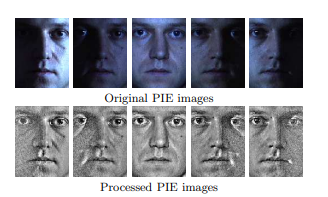
\includegraphics[width=0.5\textwidth]{beeld_voorbewerking.png}
    \caption{Beeld voorbewerking door het verwijderen van verschillende lichtinvallen. Bron: An Image Preprocessing Algorithm for Illumination Invariant Face Recognition \autocite{RalphBrajovic}}
\end{figure}


\subsection{Haar-achtige kenmerkdetectie}
Om het gezicht en de ogen te kunnen waarnemen, wordt er gebruik gemaakt van Haar-achtige kenmerkdetectie. Het meest gebruikte is AdaBoost vanwege zijn snelheid en nauwkeurigheid \autocite{Viola2004}.

Deze kenmerkdetectie houdt rekening met aangrenzende rechthoeken binnen een specifiek gebied in een bewegend detectievenster. Een afbeeldingsgebied kan omschreven worden als een combinatie van verschillende Haar-achtige kenmerken \autocite{Jibo2013}. Het aantal en types kunnen dan weer aangezien worden als verschillende objecten. De cumulatieve som van intensiteit vanaf de oorsprong wordt gedefinieerd als \begin{equation*}S_{i,j} = \sum_{x=0}^{i} \sum_{y=0}^{j} I(i, j)\end{equation*} Hierbij staat \( I_\text{(i,j)} \) voor de intensiteit op locatie (i,j), en \( S_\text{(i,j)} \) voor de cumulatieve som van intensiteiten vanaf de oorsprong op locatie (i,j). De som van intensiteit van de rechthoek, gedefinieerd als twee punten \( (x_{\text{links}}, y_{\text{boven}}) \) en  \( (x_{\text{rechts}}, y_{\text{onder}}) \), kan berekend worden volgens deze formule, die de berekening versnelt \begin{equation*}
    S_{\text{acc}}(x_{\text{rechts}}, y_{\text{onder}}) - S_{\text{acc}}(x_{\text{links}}, y_{\text{onder}}) - S_{\text{acc}}(x_{\text{rechts}}, y_{\text{boven}}) + S_{\text{acc}}(x_{\text{links}}, y_{\text{boven}})
\end{equation*}
\begin{itemize}
    \item \( S_{\text{acc}}(x_{\text{rechts}}, y_{\text{onder}}) \): Dit is de cumulatieve som van de intensiteiten tot het punt \( (x_{\text{rechts}}, y_{\text{onder}}) \). Het omvat alle pixelintensiteiten binnen en inclusief de rechthoek, vanaf de linkerbovenhoek tot de rechteronderhoek.
    \item \( S_{\text{acc}}(x_{\text{links}}, y_{\text{onder}}) \): Dit is de cumulatieve som van de intensiteiten tot het punt \( (x_{\text{links}}, y_{\text{onder}}) \). Het omvat alle pixelintensiteiten binnen en inclusief de rechthoek, vanaf de linkerbovenhoek tot de linkerbenedenhoek.
    \item \( S_{\text{acc}}(x_{\text{rechts}}, y_{\text{boven}}) \): Dit is de cumulatieve som van de intensiteiten tot het punt \( (x_{\text{rechts}}, y_{\text{boven}}) \). Het omvat alle pixelintensiteiten binnen en inclusief de rechthoek, vanaf de linkerbovenhoek tot de rechterbovenhoek.
    \item \( S_{\text{acc}}(x_{\text{links}}, y_{\text{boven}}) \): Dit is de cumulatieve som van de intensiteiten tot het punt \( (x_{\text{links}}, y_{\text{boven}}) \). Het omvat alle pixelintensiteiten binnen en inclusief de rechthoek, vanaf de linkerbovenhoek tot de linkerbovenhoek.
\end{itemize}


\subsection{Gezichtsdetectie}
Het gezicht wordt gedetecteerd door de Haar-achtige kenmerkdetectie \autocite{Viola2004}. Het zwaartepunt van het gezicht wordt berekend en vervolgens gebruikt om de knik- en rotatiebewegingen te meten van het gezicht. Een knikbeweging wordt gezien als de verticale beweging van het zwaartepunt groter is dan de horizontale beweging. Een rotatiebeweging werkt andersom \autocite{Jibo2013}. Een snelheid van 100 pixels per seconde wordt gebruikt als een grenswaarde voor de hoofdbewegingen in zowel horizontale als verticale richting.
\subsection{Detecteren van het oog}
Om het oog te kunnen detecteren zijn er verschillende algoritmes, deze zijn onder andere Hough-transformatie, patroonmatching, Principle Component Analysis (PCA) en het Adaboost algoritme. Het Adaboost algoritme maakt gebruikt van de Haar-achtige kenmerkdetectie \autocite{Viola2004}. Het ooggebied ligt horizontaal tussen 1/6 en 5/6 van het gezicht, terwijl het zich verticaal meestal tussen 1/4 en 1/2 bevindt. De breedte en hoogte van het gebied, dat dient om het oog te detecteren, wordt vastgesteld door de volgende formules: \begin{equation*}W_{gebied} = W_{gezicht} \times \frac{1}{4} \end{equation*} \begin{equation*}H_{gebied} = H_{gezicht} \times \frac{1}{3} \end{equation*}
\subsection{Knipperdetectie}
Een knipper wordt gedetecteerd doordat er een verandering is van zwarte pixels in het oog. Een open oog heeft een grotere pupil, dus meer zwarte pixels, dan een gesloten oog. Het oog wordt eerst omgezet naar een binair zwart-wit afbeelding. Vervolgens wordt de ratio van het aantal zwarte pixels berekend. Tenslotte dient deze ratio als een criterium om een knipper te detecteren.
\subsection{Oordelen van vermoeidheid}
Er zijn drie criteria die dienen om de vermoeidheid te oordelen. Deze zijn de frequentie van de knik- en rotatiebewegingen en PERCLOS (Percent Eye Closed). Een vermoeide bestuurder kan last hebben van frequente knikbewegingen en vaak knipperen. PERCLOS is een belangrijk en veelgebruikte indicator om vermoeidheid te detecteren. Het wordt gedefinieerd als het percentage tijd waarin dat de ogen gesloten zijn in een korte tijd (dit is vaak 30 seconden). Een oog wordt als gesloten beschouwd indien de zichtbare pupil kleiner is dan 30\% van zijn maximale opening. PERCLOS wordt als volgt berekend: \begin{equation*}PERCLOS = \frac{N}{30\times S}\end{equation*} waarin N staat voor het aantal knipperingen in de recentste 30 seconden, S is de bemonsteringsfrequentie.


\section{Artificiële Intelligentie}
Artificiële, beter gekend als kunstmatige, intelligentie is een manier voor machines om het `gedachteproces' van een mens na te bootsen. Hiermee zijn verschillende computerprogramma's in staat om te redeneren, conclusies te vormen en te antwoorden zoals bijna ieder hedendaags persoon kan. De meest bekende kunstmatige intelligentie, die bij zowaar niemand meer onbekend blijft, is ChatGPT. Dat in staat is om vragen te beantwoorden, meer uitleg geven over verschillende programmeertalen, wiskundige formules uit te leggen en op te lossen etc. Er is een continue ontwikkeling op dit vakgebied en wordt alsmaar meer geïmplementeerd in het dagelijks leven.

\subsection{Gezichtsdetectie}
AI heeft verschillende functionaliteiten. Zo is het in staat om het gezicht te detecteren van zowel foto's, video's en in real-time. Het kan echter wel zijn dat de nauwkeurigheid en de detectieratio aangetast worden. Dit wordt gedefinieerd als 'uitdagingen', enkele van deze zijn:
\begin{itemize}
    \item \textbf{Belichting}: Dit kan niet uniform zijn. Dat wil zeggen dat er enkele delen van het desbetreffende detectieframe meer of minder belicht zijn dan het andere deel.
    \item \textbf{Oriëntatie}: De richting hoe het gezicht gepositioneerd is.
    \item \textbf{Afstand}: De afstand van het gezicht ten opzichte van de camera.
    \item \textbf{Resolutie}: De resolutie van het beeld waarin het detecteren moet gebeuren.
    \item \textbf{Blokkeringen}: Één of meerdere objecten die tussenin de camera en het gezicht staan.
    \item \textbf{Complexe achtergronden}: Er zijn te veel objecten aanwezig in de achtergrond van het detectieframe.
\end{itemize}
Deze punten zorgen er elk voor dat er een extra uitdaging komt bij het detecteren van het gezicht, waardoor de nauwkeurigheid en het detectieratio verminderen \autocite{Kumar2019}. Binnenin het gebied van gezichtsdetectie, kunnen er verschillende detectietechnieken zijn. Deze technieken hebben elk een andere aanpak over hoe dat het gezicht wordt gedetecteerd.

\subsubsection{Active Shape Model}
Het doel van Active Shape Model (ASM) is om automatisch oriëntatiepunten te lokaliseren. Deze punten dienen om een vorm te definiëren. In het geval van het gezicht, focust het zich op de neus, ogen, mond, lippen en wenkbrauwen. ASM wordt getraind doordat er een statisch gezichtsmodel wordt gebouwd, met afbeeldingen waarop handmatig de oriëntatiepunten staan. ASM kan worden onderverdeeld in 3 groepen. Deze zijn Snakes, Point Distribution Model (PDM) en deformable templates.

\paragraph{Snakes}
Het eerste type maakt gebruikt van een generieke actieve omtrek, genaamd 'Snakes' \autocite{Kass1988}.
Snakes worden gebruikt om de grenzen van het hoofd te identificeren. Om deze taak uit te voeren, wordt er eerst een 'snake' geïnitialiseerd in de buurt van een hoofdgrens. Vervolgens gaat het opzoek naar nabijgelegen randen en neemt het stilaan de vorm van het hoofd aan. De evolutie hiervan wordt bereikt door het minimaliseren van een energiefunctie. Het wordt als volgt genoteerd:
\begin{equation*}
    E_{\text{snake}} = E_{\text{internal}} +  E_{\text{external}}
\end{equation*}
waarbij \(E_{\text{internal}} \) en \(E_{\text{external}} \) de interne en externe energiefuncties zijn.
De twee algemene overwegingen voor een snake te vormen zijn de selectie van energietermen en energie minimalisatie.
Elastische energie wordt hier gebruikt als interne energie \autocite{HJELMAS}. Dit varieert met de afstand tussen de controle punten van de snake. Hierdoor wordt er een omtrek verkregen dat in staat is om te vergroten of te verkleinen. Externe energie hangt dan echter weer af van de kenmerken van het beeld. Snakes hebben echter enkele nadelen. De omtrek komt vaak vast te zitten op valse beeldkenmerken en de snakes zijn niet geschikt voor het uittrekken van niet-convexe kenmerken.

\paragraph{Point Distribution Model}
Het Point Distribution Model (PDM) is onafhankelijk ontwikkeld van geautomatiseerde beeldanalyse en heeft statische modellen van vorm \autocite{HJELMAS}. Het idee achter PDM is dat men vormen kan voorstellen als vectoren. Nadien kunnen er standaard statische methodes op toegepast worden. De modellen leren toegestane situaties van vormpunten uit trainingsvoorbeelden en gebruiken vervolgens de hoofdcomponenten om het model op te bouwen. \textcite{Yuille1992} heeft het eerste parametrische statische vormmodel van beeldanalyse, dat gebaseerd is op de hoofdcomponenten van de oriëntatiepunten hun afstanden, gepresenteerd. Het PDM kan aanschouwd worden als het basismodel van Active Shape Model.

\paragraph{Deformable Templates}